\documentclass[11pt,a4paper]{article}

\usepackage[T1]{fontenc}
\usepackage[utf8]{inputenc}
\usepackage{lmodern}
\usepackage[final]{microtype}
\usepackage[a4paper,margin=1in]{geometry}
\usepackage{amsmath,amssymb,mathtools}
\usepackage{graphicx}
\usepackage{booktabs}
\usepackage{setspace}
\usepackage[font=small,labelfont=bf,labelsep=period,skip=6pt]{caption}
\usepackage[round,authoryear]{natbib}
\usepackage{titlesec}
\usepackage{enumitem}
\usepackage{xcolor}
\usepackage[bottom,hang,flushmargin]{footmisc}
\usepackage{xurl}
\usepackage[colorlinks=true,linkcolor=linkblue,citecolor=linkblue,urlcolor=linkblue]{hyperref}

\definecolor{linkblue}{HTML}{1F4E8C}
\hypersetup{pdftitle={An Empirical Study in Junior Mining Stock Risk Management: Weak-Form Efficiency Tests and Value-at-Risk Estimation with GARCH Models},pdfauthor={Mael Tok}}
\setstretch{1.12}
\setlength{\parskip}{0pt}
\setlength{\footnotemargin}{1.2em}
\titleformat{\section}{\normalfont\large\bfseries}{\thesection}{0.8em}{}
\titleformat{\subsection}{\normalfont\normalsize\bfseries}{\thesubsection}{0.8em}{}
\titlespacing*{\section}{0pt}{1.4\baselineskip}{0.5\baselineskip}
\titlespacing*{\subsection}{0pt}{1.0\baselineskip}{0.35\baselineskip}
\setlist{itemsep=2pt,topsep=4pt}
\bibpunct{(}{)}{;}{a}{}{,}
\setlength{\bibsep}{3pt}
\setlength{\abovedisplayskip}{7pt plus 2pt minus 3pt}
\setlength{\belowdisplayskip}{7pt plus 2pt minus 3pt}
\frenchspacing
\setcounter{tocdepth}{2}

\newcommand{\E}{\mathbb{E}}
\newcommand{\Var}{\operatorname{Var}}
\newcommand{\Cov}{\operatorname{Cov}}
\newcommand{\VR}{\mathrm{VR}}
\newcommand{\ind}{\mathbf{1}}
\newcommand{\tabnote}[1]{\par\vspace{5pt}\begin{minipage}{\linewidth}\setstretch{1.0}\footnotesize\textit{Notes:} #1\end{minipage}}

% generated by code/tables.py -- do not edit
\newcommand{\nPrices}{1{,}727}
\newcommand{\nRet}{1{,}726}
\newcommand{\nUsed}{1{,}691}
\newcommand{\nStale}{35}
\newcommand{\aruSD}{5.00}
\newcommand{\aruAnnVol}{79}
\newcommand{\xaoSD}{1.03}
\newcommand{\xaoAnnVol}{16}
\newcommand{\aruSkew}{1.46}
\newcommand{\aruKurt}{18.2}
\newcommand{\aruMax}{58.4}
\newcommand{\aruMin}{\ensuremath{-}26.8}
\newcommand{\aruMean}{0.027}
\newcommand{\zeroShare}{25}
\newcommand{\xaoSkew}{\ensuremath{-}1.29}
\newcommand{\capmAlpha}{0.007}
\newcommand{\capmAlphaSE}{0.103}
\newcommand{\capmAlphaT}{0.07}
\newcommand{\capmBeta}{1.11}
\newcommand{\capmBetaSE}{0.14}
\newcommand{\capmBetaT}{7.9}
\newcommand{\capmBetaOneT}{0.76}
\newcommand{\capmRsq}{5.2}
\newcommand{\capmIdio}{95}
\newcommand{\capmCorr}{0.23}
\newcommand{\capmResidSD}{4.87}
\newcommand{\rhoOne}{\ensuremath{-}0.113}
\newcommand{\rhoOneT}{\ensuremath{-}4.66}
\newcommand{\rhoOneTrob}{\ensuremath{-}3.05}
\newcommand{\rhoOneRes}{\ensuremath{-}0.134}
\newcommand{\rhoOneResTrob}{\ensuremath{-}3.51}
\newcommand{\vrTwo}{0.89}
\newcommand{\vrTwoZ}{\ensuremath{-}3.03}
\newcommand{\vrFive}{0.81}
\newcommand{\vrFiveZ}{\ensuremath{-}2.43}
\newcommand{\vrTen}{0.81}
\newcommand{\vrTenZ}{\ensuremath{-}1.66}
\newcommand{\vrTwenty}{0.82}
\newcommand{\vrTwentyZ}{\ensuremath{-}1.10}
\newcommand{\arRsq}{1.3}
\newcommand{\arMeanAbs}{0.37}
\newcommand{\meanAbsRet}{3.3}
\newcommand{\qTwoTen}{47}
\newcommand{\qTwoTenXao}{2{,}533}
\newcommand{\archLM}{23.9}
\newcommand{\xaoRhoOne}{\ensuremath{-}0.13}
\newcommand{\xaoRhoOneT}{\ensuremath{-}5.4}
\newcommand{\xaoRhoOneTrob}{\ensuremath{-}2.0}
\newcommand{\tickMean}{2.2}
\newcommand{\tickMedian}{2.0}
\newcommand{\tickMin}{0.7}
\newcommand{\tickMax}{5.0}
\newcommand{\priceMin}{0.043}
\newcommand{\priceMax}{0.68}
\newcommand{\shareBelow}{32}
\newcommand{\rollSpread}{3.4}
\newcommand{\rollLow}{1.9}
\newcommand{\rollHigh}{3.9}
\newcommand{\rhoLow}{\ensuremath{-}0.05}
\newcommand{\rhoHigh}{\ensuremath{-}0.13}
\newcommand{\tickLow}{1.5}
\newcommand{\tickHigh}{2.5}
\newcommand{\conGross}{0.35}
\newcommand{\conGrossT}{3.4}
\newcommand{\conNet}{\ensuremath{-}0.74}
\newcommand{\conNetT}{\ensuremath{-}7.1}
\newcommand{\conLoss}{0.74}
\newcommand{\conCost}{1.09}
\newcommand{\conTurn}{1.02}
\newcommand{\conBreakeven}{0.34}
\newcommand{\conHalf}{1.1}
\newcommand{\gnLL}{\ensuremath{-}5{,}020.4}
\newcommand{\gnPers}{0.935}
\newcommand{\gnHalf}{10}
\newcommand{\gnAIC}{10{,}050.9}
\newcommand{\gnBIC}{10{,}078.0}
\newcommand{\gnPhi}{\ensuremath{-}0.119}
\newcommand{\gnC}{\ensuremath{-}0.03}
\newcommand{\gnKurt}{18.6}
\newcommand{\gnZmax}{12.0}
\newcommand{\enLL}{\ensuremath{-}5{,}000.1}
\newcommand{\enPers}{0.965}
\newcommand{\enHalf}{19}
\newcommand{\enAIC}{10{,}012.2}
\newcommand{\enBIC}{10{,}044.8}
\newcommand{\enPhi}{\ensuremath{-}0.137}
\newcommand{\enC}{0.03}
\newcommand{\enKurt}{18.6}
\newcommand{\enZmax}{12.1}
\newcommand{\enGam}{0.071}
\newcommand{\enGamT}{3.6}
\newcommand{\gtLL}{\ensuremath{-}4{,}853.3}
\newcommand{\gtPers}{0.933}
\newcommand{\gtHalf}{10}
\newcommand{\gtAIC}{9{,}718.5}
\newcommand{\gtBIC}{9{,}751.1}
\newcommand{\gtPhi}{\ensuremath{-}0.126}
\newcommand{\gtC}{\ensuremath{-}0.24}
\newcommand{\gtKurt}{18.7}
\newcommand{\gtZmax}{12.2}
\newcommand{\gtNu}{3.96}
\newcommand{\etLL}{\ensuremath{-}4{,}844.0}
\newcommand{\etPers}{0.958}
\newcommand{\etHalf}{16}
\newcommand{\etAIC}{9{,}702.1}
\newcommand{\etBIC}{9{,}740.1}
\newcommand{\etPhi}{\ensuremath{-}0.133}
\newcommand{\etC}{\ensuremath{-}0.22}
\newcommand{\etKurt}{18.7}
\newcommand{\etZmax}{12.3}
\newcommand{\etNu}{4.12}
\newcommand{\etGam}{0.051}
\newcommand{\etGamT}{2.5}
\newcommand{\gsLL}{\ensuremath{-}4{,}845.1}
\newcommand{\gsPers}{0.929}
\newcommand{\gsHalf}{9}
\newcommand{\gsAIC}{9{,}704.2}
\newcommand{\gsBIC}{9{,}742.2}
\newcommand{\gsPhi}{\ensuremath{-}0.132}
\newcommand{\gsC}{\ensuremath{-}0.04}
\newcommand{\gsKurt}{18.5}
\newcommand{\gsZmax}{12.2}
\newcommand{\gsNu}{4.15}
\newcommand{\gsLam}{0.132}
\newcommand{\gsLamT}{3.8}
\newcommand{\esLL}{\ensuremath{-}4{,}836.4}
\newcommand{\esPers}{0.955}
\newcommand{\esHalf}{15}
\newcommand{\esAIC}{9{,}688.8}
\newcommand{\esBIC}{9{,}732.3}
\newcommand{\esPhi}{\ensuremath{-}0.135}
\newcommand{\esC}{\ensuremath{-}0.04}
\newcommand{\esKurt}{18.8}
\newcommand{\esZmax}{12.4}
\newcommand{\esNu}{4.30}
\newcommand{\esLam}{0.127}
\newcommand{\esLamT}{4.0}
\newcommand{\esGam}{0.055}
\newcommand{\esGamT}{2.9}
\newcommand{\gnUncond}{5.2}
\newcommand{\gnAlpha}{0.100}
\newcommand{\gnBeta}{0.835}
\newcommand{\gnOmega}{1.792}
\newcommand{\lrNormT}{312}
\newcommand{\lrTSkew}{15.3}
\newcommand{\lrTSkewG}{16.4}
\newcommand{\oosN}{941}
\newcommand{\oosWindow}{750}
\newcommand{\oosExpOne}{9.4}
\newcommand{\oosExpFive}{47.1}
\newcommand{\esQone}{\ensuremath{-}2.38}
\newcommand{\esQninenine}{2.87}
\newcommand{\etQone}{\ensuremath{-}2.65}
\newcommand{\etQninenine}{2.65}
\newcommand{\nQone}{\ensuremath{-}2.33}
\newcommand{\nQninenine}{2.33}
\newcommand{\avgVarESL}{11.9}
\newcommand{\avgVarESR}{14.0}
\newcommand{\avgVarNL}{11.7}
\newcommand{\avgVarNR}{11.9}
\newcommand{\violN}{16}
\newcommand{\violSigRank}{38}
\newcommand{\corrSigR}{0.05}
\newcommand{\esJumpLimit}{13.5}
\newcommand{\nJumpLimit}{11.6}
\newcommand{\jumpRatioN}{5}
\newcommand{\jumpKappa}{0.19}
\newcommand{\jumpTheta}{2.5}
\newcommand{\jumpDelta}{6.8}
\newcommand{\jumpThetaT}{2.8}
\newcommand{\jumpLL}{\ensuremath{-}4{,}857.3}
\newcommand{\jumpAIC}{9{,}730.6}
\newcommand{\jumpBIC}{9{,}774.0}
\newcommand{\jumpShare}{42}
\newcommand{\jumpPerYear}{48}
\newcommand{\jumpN}{123}
\newcommand{\jumpUp}{98}
\newcommand{\jumpDown}{25}
\newcommand{\jumpPers}{0.88}
\newcommand{\tickZero}{25}
\newcommand{\tickOne}{35}
\newcommand{\tickTwo}{78}
\newcommand{\rawEsUC}{0.09}
\newcommand{\rawN}{1{,}726}
\newcommand{\rawKurt}{19.6}
\newcommand{\rawSkew}{1.68}
\newcommand{\rawRhoOne}{\ensuremath{-}0.112}
\newcommand{\rawRhoOneTrob}{\ensuremath{-}3.12}
\newcommand{\rawVrTwo}{0.89}
\newcommand{\rawEsNu}{3.78}
\newcommand{\rawEsLam}{0.113}
\newcommand{\rawEsLL}{\ensuremath{-}4{,}921.7}
\newcommand{\rawGtLL}{\ensuremath{-}4{,}936.6}
\newcommand{\rawEtLL}{\ensuremath{-}4{,}928.3}
\newcommand{\rawBeta}{1.05}
\newcommand{\dmHSLOne}{\ensuremath{-}0.18}
\newcommand{\dmHSROne}{\ensuremath{-}0.03}
\newcommand{\dmHSLFive}{1.32}
\newcommand{\dmHSRFive}{0.33}
\newcommand{\dmNormalLOne}{\ensuremath{-}0.29}
\newcommand{\dmNormalROne}{0.73}
\newcommand{\dmNormalLFive}{2.73}
\newcommand{\dmNormalRFive}{0.66}
\newcommand{\dmGARCHNLOne}{\ensuremath{-}1.44}
\newcommand{\dmGARCHNROne}{1.59}
\newcommand{\dmGARCHNLFive}{2.52}
\newcommand{\dmGARCHNRFive}{2.24}
\newcommand{\dmEGARCHtLOne}{3.84}
\newcommand{\dmEGARCHtROne}{0.22}
\newcommand{\dmEGARCHtLFive}{2.19}
\newcommand{\dmEGARCHtRFive}{0.14}


\begin{document}

% ------------------------------------------------------------------ title page
\hypersetup{pageanchor=false}
\begin{titlepage}
\setstretch{1.1}
\vspace*{1.2cm}
\begin{center}
{\LARGE\bfseries An Empirical Study in Junior Mining Stock\\[4pt] Risk Management\par}
\vspace{0.45cm}
{\Large Weak-Form Efficiency Tests and Value-at-Risk Estimation\\[2pt] with GARCH Models\par}
\vspace{1.1cm}
{\large Mael Tok\footnote{This paper originated in a voluntary research internship at the Faculty of Economics of the University of Montpellier in June 2025, supervised by Dr.\ Roman Mestre. He taught me the methods used here, and the empirical work on which the paper is based was carried out jointly with him; see the statement of contributions at the end of the paper. I thank him for his guidance. The paper was revised and extended in 2026, while I was an undergraduate student at McGill University. Code: \url{https://github.com/2008MT/aru-garch-var}.}}\\[4pt]
{\normalsize McGill University}\\[0.9cm]
{\normalsize This version: November 2026\\ First version: December 2025}
\end{center}
\vspace{1.0cm}

\begin{center}\textbf{Abstract}\end{center}
\vspace{-2pt}
\begin{quote}
\setstretch{1.1}\small
This paper studies the daily risk of Arafura Rare Earths (ASX:\ ARU), a pre-production rare-earth developer, between August 2018 and June 2025. I first ask whether its returns are predictable. They show a negative first-order autocorrelation of \rhoOne{} that remains significant under heteroskedasticity-robust inference, but closing quotes show that it is bid--ask bounce on a coarse price grid: the closing price sits at the bid or the ask on \qAtQuote\% of days, the autocorrelation is insignificant when returns are measured at quote mid-points, and a contrarian trading rule built on it loses money once the quoted spread is paid. I therefore find no exploitable departure from weak-form efficiency. What is predictable is risk. I fit AR(1)--GARCH and EGARCH models with Normal, Student-$t$ and skewed-$t$ innovations, and a GARCH model with Poisson jumps, and evaluate their one-day Value-at-Risk forecasts out of sample for long and short positions. The decisive modelling choice is the shape of the innovation distribution rather than the volatility recursion. Tails are heavy (four to five degrees of freedom) and asymmetric, with the largest moves on the upside, as expected of an equity that is in effect an option on an unbuilt project: Gaussian models understate the short seller's risk, symmetric Student-$t$ models overstate the long holder's, and the skewed-$t$ and jump models are correctly calibrated in both tails.
\end{quote}
\vspace{0.5cm}
\noindent{\small\textbf{Keywords:} market efficiency, bid--ask bounce, tick size, GARCH, EGARCH, skewed Student-$t$, Poisson jumps, Value-at-Risk, backtesting, rare earths.}\\[3pt]
\noindent{\small\textbf{JEL classification:} C22, C58, G14, G32.}
\end{titlepage}
\hypersetup{pageanchor=true}
\setcounter{footnote}{0}
\pagenumbering{roman}
{\setstretch{1.05}\hypersetup{linkcolor=black}\tableofcontents}
\clearpage
\pagenumbering{arabic}

% ------------------------------------------------------------------ 1
\section{Introduction}

Neodymium and praseodymium (NdPr) are the rare-earth elements used in the permanent magnets of electric-vehicle motors and wind turbines. Arafura Rare Earths Ltd (ASX:\ ARU) is developing the Nolans NdPr project in Australia's Northern Territory, with a design capacity of 4,440 tonnes of NdPr oxide a year and a capital cost to first production estimated at about A\$1.7 billion.\footnote{Figures from \citet{arafura2023}.} The company is not yet in production. Its share price is in effect a claim on a project that is not yet financed or built, so it reacts to commodity prices, to geopolitics, and above all to financing news. Over the sample studied here the stock traded between A\$\priceMin{} and A\$\priceMax{}, with an annualised volatility of about \aruAnnVol\%, roughly five times that of the Australian market index.

This paper asks two questions about that risk. The first is whether the stock's daily return can be predicted from its own past, which is the question of weak-form efficiency \citep{fama1970}. The second is how well standard conditional-volatility models forecast the one-day Value-at-Risk (VaR) of a position in the stock, and which modelling choices matter for that forecast.

The two questions are sometimes linked by the argument that a risk model built on past returns is only justified if the market is \emph{in}efficient. Separating them is the organising idea of the paper. Weak-form efficiency restricts the conditional \emph{mean} of returns: past prices should not help to forecast future returns beyond a fair compensation for risk. It places no restriction on the conditional variance or on the shape of the return distribution. Volatility clustering and fat tails are found in almost every financial return series \citep{cont2001}, including those of markets nobody regards as inefficient. A VaR model exploits predictability in \emph{risk}, which is compatible with an efficient market.

The main findings are three.

\begin{enumerate}[leftmargin=1.4em]
\item \emph{The return is serially correlated, but not exploitably so.} The first-order autocorrelation of daily returns is \rhoOne{} and is statistically significant. Its source is the trading mechanism. The minimum price step is on average \tickMean\% of the share price, and the closing price is recorded at the bid or at the ask on \qAtQuote\% of days, which produces exactly this pattern \citep{roll1984}. Measured at the mid-point of the closing quotes, the autocorrelation falls to \midRho{} and is no longer significant. A trading rule that bets on the reversal earns \conGross\% a day at closing prices, nothing at mid-quotes, and loses \conLoss\% a day when it buys at the ask and sells at the bid.
\item \emph{Risk is predictable, and its shape matters more than its dynamics.} The largest gain in fit comes from the innovation distribution. Tails are heavy, with four to five degrees of freedom, and asymmetric: large moves are mostly upward, as on 14 March 2024, when the share price rose \jumpSimple\% in a day after the Australian Government announced an A\$840 million funding package for Nolans.\footnote{See \citet{miningweekly2024}. The corresponding log-return is \jumpLog\%.} A skewed Student-$t$ distribution \citep{hansen1994} is preferred to the symmetric one, and a Poisson jump model estimates that more than four in five of the stock's jumps are upward.
\item \emph{Out of sample, the tail asymmetry decides which VaR models work.} Over \oosN{} one-day forecasts, Gaussian models produce about twice the expected number of 1\% violations for a short position while being too conservative for a long one. Symmetric Student-$t$ models fix the first problem but not the second. Skewed-$t$ and jump models pass every coverage test. So does plain historical simulation: for this stock, volatility dynamics add little once the shape of the distribution is right.
\end{enumerate}

These results have an economic reading, developed in Section~\ref{sec:disc}. The equity of a company whose only asset is an unfinanced project behaves like an option on that project: its value is convex in news about financing, so good news arrives as large upward jumps. Stocks with this lottery-like profile are known to attract investors who pay for positive skewness \citep{barberishuang2008,bali2011}, and the party who bears the jump risk is the short seller, which is the risk that a Gaussian model understates.

The paper is a case study of a single stock, and its conclusions should not be generalised without evidence from other junior resource companies. Section~\ref{sec:data} describes the data. Section~\ref{sec:eff} examines return predictability. Section~\ref{sec:vol} presents and estimates the volatility models, Section~\ref{sec:var} evaluates their VaR forecasts, Section~\ref{sec:disc} interprets the results and discusses limitations, and Section~\ref{sec:concl} concludes.

% ------------------------------------------------------------------ 2
\section{Data}\label{sec:data}

\subsection{Sample and returns}

The data are from the Bloomberg Terminal: daily closing prices, closing bid and ask quotes and trading volume of ARU, and daily closing levels of the All Ordinaries index (XAO), the broad Australian equity benchmark, from 15 August 2018 to 16 June 2025. Returns are continuously compounded and expressed in per cent,
\begin{equation}
r_t = 100\,\ln\!\left(\frac{P_t}{P_{t-1}}\right),
\end{equation}
where $P_t$ is the closing price on day $t$. Arafura paid no dividends during the period. The risk-free rate used in excess returns is the daily Treasury-bill return from Kenneth French's data library; at the daily frequency it is of the order of 0.01\% and has no material effect on any result.

The sample contains \nDays{} exchange days. On \nHalt{} of them ARU was in a trading halt pending a company announcement and has no closing price. The return on the first day after a halt is measured from the last close before it, and the index and risk-free returns are measured over the same interval, which gives \nUsed{} daily returns. On every other day the stock traded: the smallest daily volume in the sample is about 97,000 shares, and the median value traded is A\$\liqMedian{} million a day. An unchanged closing price is therefore a price that did not move, never a day without trading.

\subsection{Descriptive statistics}

\begin{table}[t]
\centering
\caption{Descriptive statistics of daily log-returns}\label{tab:desc}
\small
\begin{tabular}{@{}lrrr@{}}
\toprule
 & ARU & XAO & Market-model residual \\
\midrule
Observations & 1{,}709 & 1{,}728 & 1{,}709 \\
Mean (\%) & 0.045 & 0.018 & 0.000 \\
Median (\%) & 0.000 & 0.099 & $-$0.299 \\
Standard deviation (\%) & 5.053 & 1.024 & 4.921 \\
Annualised volatility (\%) & 80.2 & 16.2 & 78.1 \\
Minimum (\%) & $-$26.83 & $-$10.01 & $-$27.68 \\
Maximum (\%) & 56.35 & 6.35 & 56.55 \\
Skewness & 1.31 & $-$1.28 & 1.41 \\
Kurtosis & 16.04 & 16.34 & 17.97 \\
Jarque--Bera & 12{,}598 & 13{,}293 & 16{,}521 \\
Zero-return days (\%) & 23.3 & 0.1 & --- \\
\bottomrule
\end{tabular}

\tabnote{Daily log-returns in per cent, 16 August 2018 to 16 June 2025. ARU is Arafura Rare Earths, with returns measured between consecutive days on which the stock traded; XAO is the All Ordinaries index on all \nIndex{} exchange days. The market-model residual is $\hat\varepsilon_t$ from equation~\eqref{eq:mm}. Annualised volatility is the daily standard deviation multiplied by $\sqrt{252}$. Kurtosis is not in excess of three (a Normal distribution has kurtosis 3). The Jarque--Bera statistic is $\chi^2(2)$ under normality (5\% critical value 5.99).}
\end{table}

\begin{figure}[t]
\centering
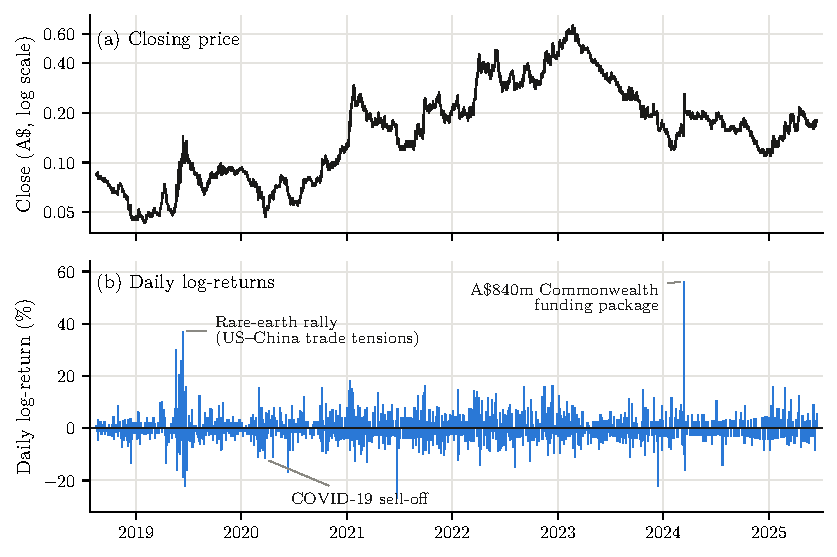
\includegraphics[width=\textwidth]{figures/fig1_price_returns.pdf}
\caption{ARU closing price and daily log-returns, August 2018 to June 2025.}\label{fig:price}
\end{figure}

Table~\ref{tab:desc} summarises the return series and Figure~\ref{fig:price} plots them. ARU's daily standard deviation is \aruSD\%, against \xaoSD\% for the index. The distribution is far from Normal: kurtosis is \aruKurt{}, and the \citet{jarquebera1987} statistic rejects normality at any level. The skewness is positive (\aruSkew{}), the opposite of the index (\xaoSkew{}). The largest moves are upward: $+\aruMax\%$ on 14 March 2024, and a cluster of gains in May and June 2019, when Chinese restrictions on rare-earth exports were widely discussed during the US--China trade dispute. The largest fall is \aruMin\%, on 24 June 2021, the first day of trading after a halt during which the company placed A\$40 million of new shares at a 29\% discount to the last close \citep{miningweekly2021}. For a developer whose value depends on a few binary events, news arrives in single announcements, and the largest of them have been good news.

\subsection{The price grid}\label{sec:grid}

A second feature of the data is less visible but matters for Section~\ref{sec:eff}. Share prices cannot take any value: the exchange fixes a minimum price step, or \emph{tick}. On the ASX the tick is A\$0.001 for shares priced below A\$0.10 and A\$0.005 for shares between A\$0.10 and A\$2.00. For most stocks a tick is a negligible fraction of the price. For ARU it is not. At a share price of A\$0.15 the nearest possible prices are A\$0.145 and A\$0.155, so the smallest change the price can record is 3.3\%.

\begin{figure}[t]
\centering
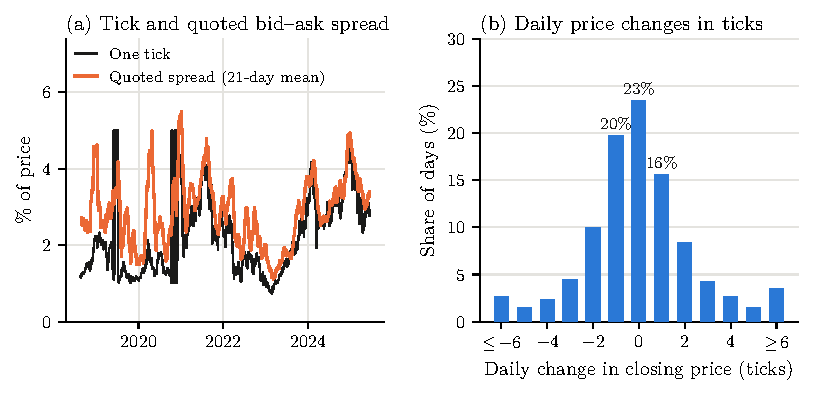
\includegraphics[width=\textwidth]{figures/fig_ticks.pdf}
\caption{The price grid. Panel (a): one tick (the minimum price step) and the bid--ask spread quoted at the close, both as a percentage of the closing price; the spread is a 21-day moving average. The jumps in the tick between about 1\% and 5\% occur when the price crosses A\$0.10 and the tick changes from A\$0.001 to A\$0.005. Panel (b): distribution of the daily change in the closing price, measured in ticks.}\label{fig:ticks}
\end{figure}

Panel (a) of Figure~\ref{fig:ticks} shows the tick as a percentage of the price over the sample. It ranges from \tickMin\% to \tickMax\% and averages \tickMean\%, the same order of magnitude as the daily standard deviation of returns. The bid--ask spread quoted at the close cannot be narrower than one tick. It is exactly one tick on \qOneTick\% of days and averages \qSpread\% of the price. Panel (b) shows the consequence for returns. The closing price is unchanged on \tickZero\% of days and moves by exactly one tick on a further \tickOne\%; on \tickTwo\% of days it moves by two ticks or fewer. Daily returns are therefore drawn from a small set of discrete values, and a one-tick difference in where the last trade of the day happens to occur is a large return.

% ------------------------------------------------------------------ 3
\section{Is the return predictable?}\label{sec:eff}

\subsection{What weak-form efficiency does and does not imply}

Let $p_t=\ln P_t$. The random-walk hypothesis states that $p_t=\mu+p_{t-1}+\varepsilon_t$, so that the return is a constant plus an unpredictable shock. \citet{clm1997} distinguish versions of it by what is assumed about $\varepsilon_t$. In the strongest version the shocks are independent and identically distributed. In the weakest they are only required to be uncorrelated, $\Cov(\varepsilon_t,\varepsilon_{t-k})=0$ for all $k\neq 0$, which allows their variance to change over time. Weak-form efficiency in the sense of \citet{fama1970} corresponds to the weak version: past prices do not help to forecast the return. It is a statement about the conditional mean,
\begin{equation}
\E\!\left[\varepsilon_t \mid \varepsilon_{t-1},\varepsilon_{t-2},\dots\right]=0 ,
\end{equation}
and says nothing about the conditional variance $\Var(\varepsilon_t\mid\varepsilon_{t-1},\dots)$ or about normality.

Three consequences follow. First, heteroskedasticity and fat tails, which Table~\ref{tab:desc} documents, are not evidence against efficiency. Second, the usual standard errors of autocorrelations assume independent shocks, so they are invalid under the hypothesis actually being tested, and inference has to be robust to changing variance. Third, following \citet{jensen1978}, a statistical rejection matters economically only if it can be turned into profit after trading costs.

A further caveat applies to any test of efficiency. It is a joint test of efficiency and of a model for the return that investors require \citep{fama1970,fama1991}: a predictable return may be a mispricing, or a fair reward for a predictable risk, and the data alone cannot say which. At the daily horizon the problem is mild. Any plausible required return is a few hundredths of a per cent a day, against a daily standard deviation of \aruSD\%, so its variation over time cannot produce autocorrelations of the size examined here. The tests below are nevertheless run both on raw returns and on returns net of market exposure, and the choice makes little difference.

\subsection{Exposure to the market}

Predictability should be assessed on the part of the return that is specific to the stock. I therefore estimate the market model in excess returns \citep{sharpe1964},
\begin{equation}\label{eq:mm}
r_t-r_{f,t}=\alpha+\beta\,(r_{m,t}-r_{f,t})+\varepsilon_t ,
\end{equation}
where $r_{m,t}$ is the return on the index and $r_{f,t}$ the risk-free rate. Beta measures the stock's sensitivity to the market, and alpha its average return beyond what that sensitivity explains. Estimation is by ordinary least squares with \citet{neweywest1987} standard errors, which allow for heteroskedasticity and autocorrelation in $\varepsilon_t$. The estimates are $\hat\beta=\capmBeta$ (standard error \capmBetaSE) and $\hat\alpha=\capmAlpha\%$ per day (standard error \capmAlphaSE). Beta is not statistically different from one and alpha is indistinguishable from zero. The $R^2$ is only \capmRsq\%: about \capmIdio\% of the variance of ARU's return is specific to the company. This is why the remainder of the paper models the return itself, and why the results below are nearly identical for $r_t$ and for the residual $\hat\varepsilon_t$.

\subsection{Tests of serial dependence}

The sample autocorrelation at lag $k$ measures how strongly today's return is related to the return $k$ days earlier,
\begin{equation}
\hat\rho_k=\frac{\sum_{t=k+1}^{T}(r_t-\bar r)(r_{t-k}-\bar r)}{\sum_{t=1}^{T}(r_t-\bar r)^2}.
\end{equation}
If returns are independent, $\hat\rho_k$ is approximately Normal with standard error $1/\sqrt{T}$, which gives the usual $t$-statistic $t_k=\sqrt{T}\hat\rho_k$. When volatility varies over time this standard error is too small, because the days that contribute most to $\hat\rho_k$ are the few days of extreme returns. \citet{lomackinlay1988} derive a standard error that remains valid in that case; the corresponding statistic is denoted $t^{*}_k$ (Appendix~\ref{app:tests}). Two joint tests complement the individual autocorrelations. The \citet{ljungbox1978} statistic tests whether the first $m$ autocorrelations are all zero,
\begin{equation}
Q_{\mathrm{LB}}(m)=T(T+2)\sum_{k=1}^{m}\frac{\hat\rho_k^{2}}{T-k}\;\sim\;\chi^2(m),
\end{equation}
and has a robust counterpart due to \citet{lobato2001}. The variance ratio of \citet{lomackinlay1988} compares the variance of $q$-day returns with $q$ times the variance of one-day returns,
\begin{equation}
\VR(q)=\frac{\Var(r_t+r_{t-1}+\dots+r_{t-q+1})}{q\,\Var(r_t)} .
\end{equation}
Under a random walk, variance grows in proportion to the horizon and $\VR(q)=1$. A value below one means that part of each day's move is subsequently reversed.

\begin{table}[t]
\centering
\caption{Serial dependence in ARU returns}\label{tab:serial}
\small
\begin{tabular}{@{}l rrr c rrr@{}}
\toprule
 & \multicolumn{3}{c}{Returns $r_t$} & & \multicolumn{3}{c}{Market-model residuals $\hat\varepsilon_t$} \\
\cmidrule(lr){2-4}\cmidrule(l){6-8}
\multicolumn{8}{@{}l}{\textit{Panel A: Autocorrelations}} \\
 Lag $k$ & $\hat\rho_k$ & $t$ & $t^{*}$ & & $\hat\rho_k$ & $t$ & $t^{*}$ \\
\midrule
1 & $-$0.110 & $-$4.55 & $-$3.04 & & $-$0.133 & $-$5.48 & $-$3.52 \\
2 & $-$0.009 & $-$0.39 & $-$0.27 & & $-$0.002 & $-$0.08 & $-$0.06 \\
3 & 0.002 & 0.09 & 0.05 & & $-$0.007 & $-$0.28 & $-$0.16 \\
4 & $-$0.023 & $-$0.95 & $-$0.73 & & $-$0.017 & $-$0.69 & $-$0.51 \\
5 & 0.036 & 1.48 & 1.19 & & 0.037 & 1.51 & 1.21 \\
\addlinespace
\multicolumn{8}{@{}l}{\textit{Panel B: Portmanteau tests}} \\
 Lags $m$ & $Q_{\mathrm{LB}}$ & $p$ & $p^{*}$ & & $Q_{\mathrm{LB}}$ & $p$ & $p^{*}$ \\
\midrule
5 & 24.0 & $<$0.001 & 0.047 & & 32.9 & $<$0.001 & 0.015 \\
10 & 41.1 & $<$0.001 & 0.018 & & 53.3 & $<$0.001 & 0.004 \\
20 & 52.7 & $<$0.001 & 0.074 & & 68.6 & $<$0.001 & 0.012 \\
\addlinespace
\multicolumn{8}{@{}l}{\textit{Panel C: Variance ratios}} \\
 Horizon $q$ & $\mathrm{VR}(q)$ & $z$ & $z^{*}$ & & $\mathrm{VR}(q)$ & $z$ & $z^{*}$ \\
\midrule
2 & 0.891 & $-$4.52 & $-$3.02 & & 0.868 & $-$5.45 & $-$3.50 \\
5 & 0.808 & $-$3.62 & $-$2.42 & & 0.776 & $-$4.22 & $-$2.71 \\
10 & 0.827 & $-$2.12 & $-$1.45 & & 0.791 & $-$2.56 & $-$1.69 \\
20 & 0.853 & $-$1.22 & $-$0.89 & & 0.827 & $-$1.44 & $-$1.01 \\
\addlinespace
\multicolumn{8}{@{}l}{\textit{Panel D: Dependence in squared series}} \\
 & Statistic & $p$ & & & Statistic & $p$ & \\
\midrule
Ljung--Box $Q^2(10)$ & 71.5 & $<$0.001 & & & 74.7 & $<$0.001 & \\
ARCH-LM(5) & 40.7 & $<$0.001 & & & 41.4 & $<$0.001 & \\
\bottomrule
\end{tabular}

\tabnote{$T=\nUsed$. Panel A: sample autocorrelations; $t$ uses the standard error $1/\sqrt{T}$, valid under independence, and $t^{*}$ the heteroskedasticity-robust standard error. Panel B: Ljung--Box statistic with its $p$-value, and the $p$-value $p^{*}$ of the robust statistic. Panel C: variance ratios with overlapping $q$-day returns; $z$ and $z^{*}$ are the test statistics under homoskedasticity and heteroskedasticity (standard Normal under the random walk). Panel D: Ljung--Box statistic on squared demeaned series and the LM test of \citet{engle1982} with five lags.}
\end{table}

\begin{figure}[t]
\centering
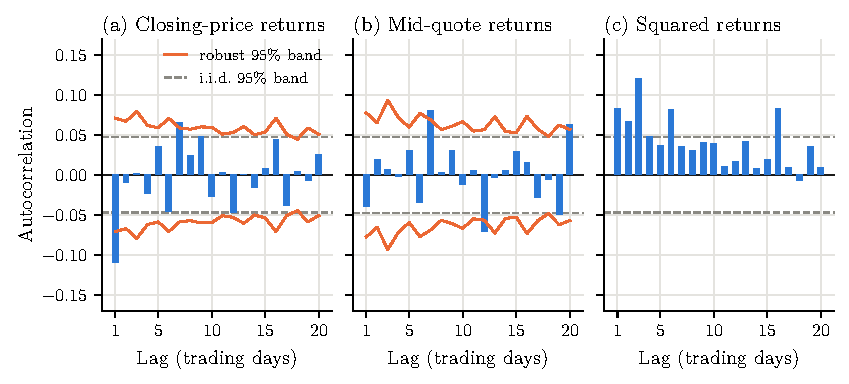
\includegraphics[width=\textwidth]{figures/fig2_acf.pdf}
\caption{Sample autocorrelations of ARU daily returns measured at closing prices and at the mid-point of the closing bid and ask, and of squared closing-price returns. Bars outside a band are significant at the 5\% level. The dashed band is $\pm1.96/\sqrt{T}$, valid under independence; the solid band uses heteroskedasticity-robust standard errors.}\label{fig:acf}
\end{figure}

Table~\ref{tab:serial} reports the results for returns and for market-model residuals, and panel (a) of Figure~\ref{fig:acf} plots the autocorrelations. The first-order autocorrelation is \rhoOne{} for returns and \rhoOneRes{} for residuals: a rise today tends to be followed by a small fall tomorrow, and conversely. Robust inference matters. The $t$-statistic at lag one falls from \rhoOneT{} to \rhoOneTrob{}, and the robust portmanteau $p$-values in Panel B are orders of magnitude larger than the Ljung--Box ones, although the test still rejects at ten lags. Beyond the first lag, only the seventh leaves the robust band ($\hat\rho_7=\rhoSeven$, $t^{*}=\rhoSevenTrob$). I know of no mechanism that would produce a seven-day effect, and one exceedance among nineteen further lags is not surprising, so I treat it as noise. The systematic departure from the random walk is the reversal at the first lag.\footnote{The market index illustrates how misleading the conventional statistics can be. Its first-order autocorrelation over the same period is \xaoRhoOne{} with a conventional $t$-statistic of \xaoRhoOneT{}, but a robust $t$-statistic of only \xaoRhoOneTrob{}; the estimate is dominated by a few days of extreme volatility in March 2020.}

The variance ratio is \vrTwo{} at two days ($z^{*}=\vrTwoZ$) and \vrFive{} at five days ($z^{*}=\vrFiveZ$), and \vrTen{} and \vrTwenty{} at ten and twenty days. If the only departure from a random walk were a first-order autocorrelation $\rho_1$, the variance ratio would be $1+2\rho_1(q-1)/q$, that is \vrImpFive, \vrImpTen{} and \vrImpTwenty{} at horizons of five, ten and twenty days. The estimates are close to these values and, if anything, drift back towards one at longer horizons. There is no additional reversal beyond the first day, as there would be if prices overreacted to news and corrected slowly.

Panel D confirms that squared returns are serially dependent: large moves tend to be followed by large moves of either sign. This is the predictability in risk that Sections~\ref{sec:vol} and~\ref{sec:var} use. It is weaker than might be expected: the Ljung--Box statistic on squared returns at ten lags is \qTwoTen{}, against \qTwoTenXao{} for the index over the same period.

\subsection{Bid--ask bounce}

A one-day reversal with no longer-horizon structure is the signature of measurement noise in the closing price. At any moment a stock has two prices: the \emph{ask}, at which one can buy, and the lower \emph{bid}, at which one can sell. Their difference is the spread. The closing price is the price of the last trade of the day, which is at the ask if that trade was a purchase and at the bid if it was a sale. Suppose the value of the stock does not change for two days, and the last trade is a purchase on the first day and a sale on the second. The recorded closing price falls by the spread although nothing has happened. A close at the ask can only be followed by an unchanged or lower recorded price, and a close at the bid by an unchanged or higher one, so recorded returns are negatively autocorrelated even when the true value follows a random walk.

\citet{roll1984} formalises this. Let the observed log price be $p_t=m_t+\tfrac{s}{2}q_t$, where $m_t$ is the efficient price, which follows a random walk with shocks $u_t$, $s$ is the proportional spread, and $q_t=\pm1$ with equal probability according to whether the last trade is a purchase or a sale. Then $\Delta p_t=u_t+\tfrac{s}{2}(q_t-q_{t-1})$ and
\begin{equation}
\Cov(\Delta p_t,\Delta p_{t-1})=-\frac{s^{2}}{4}\qquad\Longrightarrow\qquad \hat s=2\sqrt{-\widehat{\Cov}(r_t,r_{t-1})} .
\end{equation}
Rounding prices to a grid has the same effect \citep{gottliebkalay1985,harris1990}. For ARU the spread implied by the autocovariance of returns is $\hat s=\rollSpread\%$. The spread actually quoted at the close averages \qSpread\% (Section~\ref{sec:grid}). An estimate obtained from closing prices alone thus recovers a spread close to the one observed in the market, which is what the model predicts if the autocorrelation is bounce and nothing else.

\begin{table}[t]
\centering
\caption{Autocorrelation and bid--ask spread by tick-size regime}\label{tab:tick}
\small
\begin{tabular}{@{}lrrrr@{}}
\toprule
Price regime (previous close) & Days & Mean tick/price (\%) & $\hat\rho_1$ & Roll spread (\%) \\
\midrule
Below A\$0.10 \;(tick A\$0.001) & 549 & 1.54 & $-$0.051 & 1.90 \\
A\$0.10 and above \;(tick A\$0.005) & 1{,}141 & 2.52 & $-$0.131 & 3.87 \\
\midrule
Full sample & 1{,}690 & 2.19 & $-$0.113 & 3.36 \\
\bottomrule
\end{tabular}

\tabnote{Days are classified by the previous day's closing price, which determines the tick: A\$0.001 below A\$0.10 and A\$0.005 from A\$0.10. Tick/price is the average of the tick divided by the closing price. The quoted spread is the average of the closing ask minus the closing bid, divided by their mid-point. $\hat\rho_1$ is the correlation between $r_t$ and $r_{t-1}$ within each regime, for returns measured at closing prices and at quote mid-points (Section~\ref{sec:quotes}). The Roll spread is $2\sqrt{-\widehat{\Cov}(r_t,r_{t-1})}$.}
\end{table}

Table~\ref{tab:tick} provides a further check. If the autocorrelation comes from the grid, it should be stronger where the grid is coarser relative to the price. It is: when the stock trades below A\$0.10, where the tick averages \tickLow\% of the price, the autocorrelation is \rhoLow{}; at A\$0.10 and above, where the tick averages \tickHigh\%, it is \rhoHigh{}. The implied spread rises from \rollLow\% to \rollHigh\%, in the same direction as the quoted spread (\qLowSpread\% and \qHighSpread\%). With these sample sizes the difference between the two autocorrelations is not statistically significant on its own, but its direction is the one the bounce explanation predicts.

\subsection{A direct test with closing quotes}\label{sec:quotes}

The evidence so far is indirect, because it infers the spread from the returns. The closing bid and ask allow two direct checks, reported in Table~\ref{tab:quotes}.

\begin{table}[t]
\centering
\caption{Closing prices and quote mid-points}\label{tab:quotes}
\small
\begin{tabular}{@{}l rr@{}}
\toprule
\multicolumn{3}{@{}l}{\textit{Panel A: Closing quotes}} \\
\midrule
Quoted spread, mean (\% of mid-quote) & \multicolumn{2}{r}{2.88} \\
Quoted spread, median (\%) & \multicolumn{2}{r}{2.67} \\
Days with a spread of one tick / two ticks / more (\%) & \multicolumn{2}{r}{69 / 23 / 8} \\
Close at the bid / at the ask / elsewhere (\%) & \multicolumn{2}{r}{50 / 35 / 15} \\
\addlinespace
\multicolumn{3}{@{}l}{\textit{Panel B: Serial dependence of daily returns}} \\
 & Closing price & Mid-quote \\
\midrule
Standard deviation (\%) & 4.84 & 4.41 \\
$\hat\rho_1$ & $-$0.106 & $-$0.040 \\
\quad robust $t^{*}$ & $-$2.88 & $-$1.00 \\
$\mathrm{VR}(2)$ & 0.894 & 0.961 \\
\quad robust $z^{*}$ & $-$2.86 & $-$0.97 \\
$\mathrm{VR}(5)$ & 0.849 & 0.970 \\
\quad robust $z^{*}$ & $-$1.93 & $-$0.36 \\
Robust portmanteau $Q^{*}(5)$, $p$-value & 0.116 & 0.798 \\
\addlinespace
\multicolumn{3}{@{}l}{\textit{Panel C: Contrarian rule, average return (\% per day)}} \\
 & Return & $t$-statistic \\
\midrule
Valued at closing prices & 0.34 & 3.24 \\
Valued at mid-quotes & $-$0.06 & $-$0.60 \\
Buying at the ask and selling at the bid & $-$1.52 & $-$14.89 \\
\bottomrule
\end{tabular}

\tabnote{Panel A: closing bid and ask on the \qNdays{} trading days with a valid quote (bid below ask). Panel B: daily log-returns measured at closing prices and at the mid-point of the closing bid and ask, on the same \qNmid{} days; $t^{*}$ and $z^{*}$ are the heteroskedasticity-robust statistics of Table~\ref{tab:serial}, and $Q^{*}(5)$ is the robust portmanteau test with five lags. Panel C: the contrarian rule of Section~\ref{sec:trade}, valued in three ways.}
\end{table}

The first check is where the closing price lies. It equals the closing bid on \qAtBid\% of days and the closing ask on \qAtAsk\%. On \qAtQuote\% of days, therefore, the recorded close is one of the two quotes and not a value between them, and which of the two depends on whether the last trade of the day was a sale or a purchase. This is the mechanism described above, observed directly.

The second check removes the bounce. The mid-point of the bid and the ask, $m_t=\tfrac12(\text{bid}_t+\text{ask}_t)$, does not depend on the side of the last trade, so returns computed from it, $r^{m}_t=100\ln(m_t/m_{t-1})$, should be free of the effect. Panel (b) of Figure~\ref{fig:acf} plots their autocorrelations. On the days for which both returns are available, the first-order autocorrelation is \sameRho{} at closing prices ($t^{*}=\sameRhoTrob$) and \midRho{} at mid-quotes ($t^{*}=\midRhoTrob$).\footnote{Mid-quote returns require a valid quote on two consecutive trading days, which leaves \qNmid{} observations. The \qInvalid{} trading days on which the closing bid is missing or not below the closing ask are dropped. They include 13 March 2024, the day before the largest return in the sample.} About \midDrop\% of the autocorrelation disappears, and what remains is not statistically different from zero. The two-day variance ratio rises from \sameVrTwo{} to \midVrTwo{}, and the robust portmanteau test no longer comes close to rejecting ($p=\midQp$). The autocorrelation is also much smaller within each tick regime (last column of Table~\ref{tab:tick}). Mid-quote returns are also less volatile than closing-price returns: the position of the close within the spread accounts for about \qNoise\% of the variance of daily returns. The small negative autocorrelation that remains may itself reflect rounding, since the quotes are also confined to the grid.

\subsection{Can the reversal be traded?}\label{sec:trade}

The economic test of efficiency is whether the pattern yields a profit. The natural strategy is a \emph{contrarian rule}, which bets each day that yesterday's move will partly reverse. Let $w_t$ be the position held during day $t$, in units of the stock:
\begin{equation}
w_t=-\operatorname{sign}(r_{t-1})=
\begin{cases}
+1 \ \text{(buy)} & \text{if the price fell yesterday,}\\
\phantom{+}0 \ \text{(no position)} & \text{if it was unchanged,}\\
-1 \ \text{(sell short)} & \text{if it rose.}
\end{cases}
\end{equation}
The position is opened at yesterday's close and valued at today's. Panel C of Table~\ref{tab:quotes} values the same rule in three ways. At closing prices its return is $w_t r_t$, which averages \conGross\% a day ($t$-statistic \conGrossT), or about \conAnn\% a year. At mid-quotes it is $w_t r^{m}_t$, which averages \conMid\% a day ($t$-statistic \conMidT): the profit is not there. The rule tends to buy after the price has closed at the bid and to sell after it has closed at the ask, so the gain it appears to make is the spread it would have had to pay. A trader cannot in fact buy at the bid or sell at the ask. Buying at the ask and selling at the bid costs half the quoted spread on each unit traded, relative to the mid-quote. The rule changes its position by \conTurn{} units a day on average and the quoted half-spread averages \conHalf\%, so that
\begin{equation*}
\underbrace{\conMid\%}_{\text{at mid-quotes}}-\underbrace{\conCost\%}_{\text{half-spread paid}}=\conNet\%\ \text{a day}\qquad(t\text{-statistic }{\conNetT}).
\end{equation*}

\subsection{Limits to arbitrage}\label{sec:arb}

The contrarian rule fails for a mechanical reason, but the costs it runs into matter more generally. \citet{shleifervishny1997} point out that arbitrage requires capital and bears risk, so that a price can stay away from fundamental value when trading against it is costly. ARU is a stock in which it is. A round trip costs the quoted spread, \qSpread\% on average, which is close to the mean absolute daily return of \meanAbsRet\%. The median value traded is A\$\liqMedian{} million a day, so a position of institutional size could not be opened or closed at the quoted prices. Selling short requires borrowing the shares, at a cost that is not observed here. Any pattern in returns smaller than these costs could persist without being traded away, and tests on returns cannot detect it. What the evidence supports is therefore efficiency in the sense of \citet{jensen1978}: no strategy based on past prices earns a profit after costs. It does not show that the price equals fundamental value at every moment, which no test of this kind could establish.

I conclude that ARU's returns reject the random walk statistically, but that the rejection reflects how prices are recorded and offers no profit. In the sense that matters economically, the evidence is consistent with weak-form efficiency.

% ------------------------------------------------------------------ 4
\section{Volatility models}\label{sec:vol}

\subsection{Conditional mean and variance}

The return is decomposed into a predictable mean and a shock whose standard deviation $\sigma_t$, the conditional volatility, depends on information available the day before:
\begin{equation}\label{eq:mean}
r_t=c+\phi\,r_{t-1}+\varepsilon_t,\qquad \varepsilon_t=\sigma_t z_t,\qquad z_t\sim\text{i.i.d. } D(0,1).
\end{equation}
The AR(1) term $\phi\,r_{t-1}$ absorbs the first-order reversal documented above. The standardised innovation $z_t$ has mean zero and variance one, and its distribution $D$ is discussed in Section~\ref{sec:dist}. Two specifications of $\sigma_t^2$ are compared.

\emph{GARCH.} The GARCH(1,1) model of \citet{bollerslev1986}, which generalises the ARCH model of \citet{engle1982}, is
\begin{equation}\label{eq:garch}
\sigma_t^2=\omega+\alpha\,\varepsilon_{t-1}^2+\beta\,\sigma_{t-1}^2,\qquad \omega>0,\ \ \alpha\ge 0,\ \ \beta\ge 0 .
\end{equation}
Today's variance is a baseline $\omega$, plus a reaction $\alpha$ to the size of yesterday's shock, plus a fraction $\beta$ of yesterday's variance. A large shock of either sign raises volatility, and the effect decays gradually, which produces volatility clustering. If $\alpha+\beta<1$ the process is covariance stationary with long-run variance
\begin{equation}
\bar\sigma^2=\E[\sigma_t^2]=\frac{\omega}{1-\alpha-\beta},
\end{equation}
and the deviation of expected variance from $\bar\sigma^2$ shrinks by the factor $\alpha+\beta$ each day: $\E_t[\sigma_{t+k}^2]-\bar\sigma^2=(\alpha+\beta)^{k-1}(\sigma_{t+1}^2-\bar\sigma^2)$. The sum $\alpha+\beta$ is called the persistence, and the half-life of a volatility shock is $\ln 0.5/\ln(\alpha+\beta)$ days.

\emph{EGARCH.} The exponential GARCH(1,1) of \citet{nelson1991} models the logarithm of the variance:
\begin{equation}\label{eq:egarch}
\ln\sigma_t^2=\omega+\alpha\left(|z_{t-1}|-\E|z_{t-1}|\right)+\gamma\,z_{t-1}+\beta\,\ln\sigma_{t-1}^2 .
\end{equation}
Because $\sigma_t^2=\exp(\cdot)$ is positive for any parameter values, no sign restrictions are needed, and persistence is measured by $\beta$ alone. The term in $\alpha$ is the response to the size of the shock, as in GARCH. The term in $\gamma$ is the response to its sign: a positive shock $z_{t-1}=+1$ changes $\ln\sigma_t^2$ by $\alpha(1-\E|z|)+\gamma$ and a negative shock $z_{t-1}=-1$ by $\alpha(1-\E|z|)-\gamma$. For equity indices $\gamma$ is typically negative, the leverage effect of \citet{black1976}: volatility rises more after falls than after gains.

\subsection{Innovation distributions}\label{sec:dist}

Three distributions are considered for $z_t$, each with mean zero and variance one.

\emph{Normal.} The standard Normal density is
\begin{equation}
f_N(z)=\frac{1}{\sqrt{2\pi}}\exp\!\left(-\frac{z^{2}}{2}\right).
\end{equation}
Its tails decay very quickly: a move of more than four standard deviations has probability $6\times10^{-5}$, about one trading day in 60 years.

\emph{Student-$t$.} Following \citet{bollerslev1987}, the Student-$t$ density with $\nu>2$ degrees of freedom, scaled to unit variance, is
\begin{equation}\label{eq:t}
f_t(z;\nu)=\frac{\Gamma\!\left(\frac{\nu+1}{2}\right)}{\sqrt{\pi(\nu-2)}\;\Gamma\!\left(\frac{\nu}{2}\right)}\left(1+\frac{z^{2}}{\nu-2}\right)^{-\frac{\nu+1}{2}} .
\end{equation}
Its tails decay as a power of $z$, so extreme moves are far more likely than under the Normal. The smaller $\nu$, the heavier the tails; as $\nu\to\infty$ the density converges to the Normal. The kurtosis is $3+6/(\nu-4)$ and is finite only for $\nu>4$.

\emph{Skewed Student-$t$.} The density of \citet{hansen1994} adds a parameter $\lambda\in(-1,1)$ that makes one tail heavier than the other:
\begin{equation}\label{eq:skt}
f_{st}(z;\nu,\lambda)=
bc\left[1+\frac{1}{\nu-2}\left(\frac{bz+a}{1+\operatorname{sign}(z+a/b)\,\lambda}\right)^{2}\right]^{-\frac{\nu+1}{2}},
\end{equation}
\begin{equation*}
c=\frac{\Gamma\!\left(\frac{\nu+1}{2}\right)}{\sqrt{\pi(\nu-2)}\;\Gamma\!\left(\frac{\nu}{2}\right)},\qquad a=4\lambda c\,\frac{\nu-2}{\nu-1},\qquad b^{2}=1+3\lambda^{2}-a^{2}.
\end{equation*}
With $\lambda>0$ the right tail is heavier, with $\lambda<0$ the left, and $\lambda=0$ gives back the symmetric density~\eqref{eq:t}.

\subsection{Estimation}

Combining the two variance equations with the three distributions gives six models. Each is estimated by maximum likelihood: the parameters are chosen to make the observed returns as probable as possible under the model. Since $\varepsilon_t=\sigma_t z_t$, the density of $r_t$ given the past is $f_D(z_t)/\sigma_t$, and the log-likelihood of the sample is
\begin{equation}\label{eq:ll}
\ln L(\vartheta)=\sum_{t=2}^{T}\left[\ln f_D\!\left(\frac{\varepsilon_t}{\sigma_t}\right)-\frac{1}{2}\ln\sigma_t^{2}\right],\qquad \varepsilon_t=r_t-c-\phi\,r_{t-1},
\end{equation}
where $\vartheta$ collects all parameters and $\sigma_t^2$ is computed recursively from~\eqref{eq:garch} or~\eqref{eq:egarch}. Standard errors are those of \citet{bollerslevwooldridge1992}, which remain valid when the assumed distribution is wrong. Models are compared by the Akaike and Bayesian information criteria, $\mathrm{AIC}=-2\ln L+2k$ and $\mathrm{BIC}=-2\ln L+k\ln T$, which reward fit and penalise the number of parameters $k$; lower values are better.\footnote{Computations use Python with the \texttt{statsmodels} library and the \texttt{arch} package of Kevin Sheppard (version 9.0). Returns on either side of a trading halt are treated as adjacent observations. In the software, $\E|z_{t-1}|$ in~\eqref{eq:egarch} is set to its Gaussian value $\sqrt{2/\pi}$ for every distribution, which affects only the constant $\omega$ (Appendix~\ref{app:absz}).}

\subsection{Estimates}

\begin{table}[t]
\centering
\caption{AR(1)--GARCH and AR(1)--EGARCH estimates}\label{tab:models}
\small
\begin{tabular}{@{}l rr rr rr@{}}
\toprule
 & \multicolumn{2}{c}{Normal} & \multicolumn{2}{c}{Student-$t$} & \multicolumn{2}{c}{Skewed $t$} \\
\cmidrule(lr){2-3}\cmidrule(lr){4-5}\cmidrule(l){6-7}
 & GARCH & EGARCH & GARCH & EGARCH & GARCH & EGARCH \\
\midrule
\multicolumn{7}{@{}l}{\textit{Panel A: Parameter estimates}} \\
$c$ & $-$0.033 & 0.035 & $-$0.235 & $-$0.220 & $-$0.039 & $-$0.035 \\
 & (0.117) & (0.123) & (0.089) & (0.090) & (0.100) & (0.104)\rlap{$^{\dagger}$} \\
$\phi$ & $-$0.119 & $-$0.137 & $-$0.126 & $-$0.133 & $-$0.132 & $-$0.135 \\
 & (0.029) & (0.028) & (0.024) & (0.024) & (0.025) & (0.022)\rlap{$^{\dagger}$} \\
$\omega$ & 1.792 & 0.122 & 1.848 & 0.140 & 1.861 & 0.151 \\
 & (0.724) & (0.025) & (0.740) & (0.042) & (0.676) & (0.042) \\
$\alpha$ & 0.100 & 0.110 & 0.120 & 0.142 & 0.117 & 0.141 \\
 & (0.033) & (0.035) & (0.032) & (0.036) & (0.028) & (0.034) \\
$\gamma$ &  & 0.071 &  & 0.051 &  & 0.055 \\
 &  & (0.020) &  & (0.020) &  & (0.019) \\
$\beta$ & 0.835 & 0.965 & 0.813 & 0.958 & 0.812 & 0.955 \\
 & (0.037) & (0.009) & (0.049) & (0.013) & (0.045) & (0.013) \\
$\nu$ &  &  & 3.957 & 4.120 & 4.155 & 4.303 \\
 &  &  & (0.437) & (0.479) & (0.481) & (0.518) \\
$\lambda$ &  &  &  &  & 0.132 & 0.127 \\
 &  &  &  &  & (0.035) & (0.031) \\
\addlinespace
\multicolumn{7}{@{}l}{\textit{Panel B: Volatility dynamics and fit}} \\
Persistence & 0.935 & 0.965 & 0.933 & 0.958 & 0.929 & 0.955 \\
Half-life (days) & 10.3 & 19.2 & 10.0 & 16.1 & 9.4 & 14.9 \\
Log-likelihood & $-$5{,}020.4 & $-$5{,}000.1 & $-$4{,}853.3 & $-$4{,}844.0 & $-$4{,}845.1 & $-$4{,}836.4 \\
Parameters & 5 & 6 & 6 & 7 & 7 & 8 \\
AIC & 10{,}050.9 & 10{,}012.2 & 9{,}718.5 & 9{,}702.1 & 9{,}704.2 & 9{,}688.8 \\
BIC & 10{,}078.0 & 10{,}044.8 & 9{,}751.1 & 9{,}740.1 & 9{,}742.2 & 9{,}732.3 \\
\addlinespace
\multicolumn{7}{@{}l}{\textit{Panel C: Diagnostics on standardised residuals ($p$-values)}} \\
Ljung--Box $Q(10)$ & 0.089 & 0.047 & 0.088 & 0.066 & 0.078 & 0.060 \\
Ljung--Box $Q^2(10)$ & 1.000 & 1.000 & 0.999 & 1.000 & 0.999 & 1.000 \\
ARCH-LM(5) & 0.991 & 1.000 & 0.978 & 0.998 & 0.979 & 0.998 \\
\bottomrule
\end{tabular}

\tabnote{Maximum-likelihood estimates of equations~\eqref{eq:mean}--\eqref{eq:egarch} on daily log-returns in per cent; robust standard errors in parentheses. Persistence is $\alpha+\beta$ for GARCH and $\beta$ for EGARCH; the half-life is $\ln 0.5/\ln(\text{persistence})$. $T=\nGarch$. Panel C reports $p$-values of Ljung--Box tests on standardised residuals $\hat z_t$ and on $\hat z_t^2$, and of the ARCH-LM test with five lags; values above 0.05 indicate no remaining dependence.}
\end{table}

Table~\ref{tab:models} reports the estimates. Five results stand out.

\emph{Volatility dynamics.} In the Gaussian GARCH model $\hat\alpha=\gnAlpha$ and $\hat\beta=\gnBeta$, so persistence is \gnPers{}: a volatility shock loses half its effect in about \gnHalf{} trading days. The implied long-run volatility $\sqrt{\hat\omega/(1-\hat\alpha-\hat\beta)}$ is \gnUncond\% a day, against a sample standard deviation of \aruSD\%. Across models, persistence lies between 0.93 and 0.96 and the half-life between two and three trading weeks.

\emph{The mean equation.} The AR(1) coefficient is between \gnPhi{} and \enPhi{} in every model, in line with Section~\ref{sec:eff}.

\emph{Tails.} Replacing the Normal by the Student-$t$ raises the log-likelihood from \enLL{} to \etLL{} for EGARCH. Twice the difference, \lrNormT{}, is the likelihood-ratio statistic for the one additional parameter, against a 5\% critical value of 3.84. The estimated degrees of freedom lie between \gtNu{} and \esNu{}, and none is more than 1.2 standard errors above four. Since the kurtosis of a Student-$t$ is finite only for $\nu>4$, the data cannot reject that the kurtosis of the innovations is infinite, and the sample kurtosis of \aruKurt{} in Table~\ref{tab:desc} is not a stable estimate of a population quantity.

\emph{Asymmetry of the distribution.} The skewness parameter is $\hat\lambda=\esLam$ in the EGARCH model, about four standard errors from zero, and the likelihood-ratio statistic against the symmetric $t$ is \lrTSkew{} (\lrTSkewG{} for GARCH). The right tail is heavier than the left. The symmetric-$t$ models reveal the same asymmetry indirectly. Their intercept is $\hat c\approx\etC\%$ a day and statistically significant, which taken literally would be an expected return of about $-50\%$ a year. It is an artefact: a symmetric density fitted to right-skewed data is centred near the mode, below the mean. With the skewed $t$ the intercept is \esC\% and insignificant.

\emph{Asymmetry of the volatility response.} The EGARCH parameter $\gamma$ is positive in all three specifications ($\hat\gamma=\esGam$ with the skewed $t$, $t$-statistic \esGamT). Volatility rises more after positive shocks than after negative ones, the reverse of the leverage effect. This is plausible for a stock whose large moves are upward jumps followed by several days of heavy repricing, but it is estimated from few episodes and should be regarded as tentative.

On both information criteria the ranking is the same: EGARCH with skewed-$t$ innovations is preferred (AIC \esAIC, BIC \esBIC), followed by EGARCH with symmetric $t$. For each distribution, EGARCH fits better than GARCH.

\subsection{Diagnostics}

If a model is adequate, the standardised residuals $\hat z_t=\hat\varepsilon_t/\hat\sigma_t$ should show no remaining dependence and should follow the assumed distribution. Panel C of Table~\ref{tab:models} addresses the first requirement. No model leaves detectable dependence in $\hat z_t^2$, so the variance equations capture the volatility clustering. None leaves detectable autocorrelation in $\hat z_t$ itself either: the Ljung--Box $p$-values at ten lags lie between 0.13 and 0.19.

\begin{figure}[t]
\centering
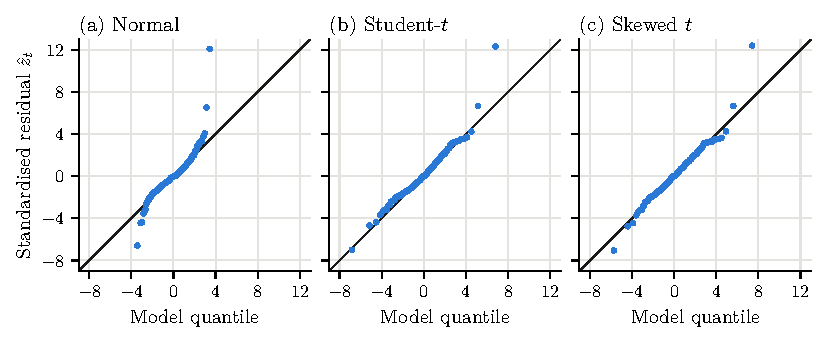
\includegraphics[width=\textwidth]{figures/fig3_qq.pdf}
\caption{Quantile--quantile plots of EGARCH standardised residuals against the fitted innovation distribution. Each point pairs an observed residual with the value the model predicts for an observation of that rank; points on the 45-degree line indicate agreement between model and data.}\label{fig:qq}
\end{figure}

Figure~\ref{fig:qq} addresses the second requirement by plotting the ordered residuals of the three EGARCH models against the quantiles of their assumed distributions. The Normal fails in both tails: observed extremes are larger than the model allows. The two $t$ distributions fit well up to about four standard deviations, with the skewed $t$ closer in the upper tail. One observation is far from the line in every panel: 14 March 2024, with a standardised residual of \esZmax. The Gaussian model treats a move of that size as impossible. The skewed-$t$ model assigns it a probability of about $3.4\times10^{-5}$, or one day in roughly 120 years. Announcement days of this kind behave like jumps, which motivates the next specification.

\subsection{A specification with Poisson jumps}\label{sec:jump}

The models above describe every return as a draw from one continuous distribution whose scale $\sigma_t$ evolves smoothly. An alternative, following \citet{merton1976} and \citet{jorion1988}, treats news days explicitly as jumps. The shock is the sum of an ordinary Gaussian component and a random number $N_t$ of jumps:
\begin{equation}\label{eq:jump}
\varepsilon_t=\sqrt{h_t}\,z_t+\sum_{j=1}^{N_t}J_{j}-\kappa\theta,\qquad z_t\sim N(0,1),\quad N_t\sim\text{Poisson}(\kappa),\quad J_{j}\sim N(\theta,\delta^{2}).
\end{equation}
The number of jumps on a day follows a Poisson distribution, $\Pr(N_t=n)=e^{-\kappa}\kappa^{n}/n!$, so $\kappa$ is the expected number of jumps a day. Each jump has mean size $\theta$ and standard deviation $\delta$. Subtracting $\kappa\theta$ keeps the mean of $\varepsilon_t$ at zero. The variance of the ordinary component follows a GARCH(1,1), $h_t=\omega+\alpha\varepsilon_{t-1}^2+\beta h_{t-1}$. Given $N_t=n$, the shock is Normal with mean $(n-\kappa)\theta$ and variance $h_t+n\delta^2$, so its density is a Poisson-weighted mixture of Normal densities,
\begin{equation}\label{eq:jumpdens}
f(\varepsilon_t)=\sum_{n=0}^{\infty}\frac{e^{-\kappa}\kappa^{n}}{n!}\;\frac{1}{\sqrt{2\pi(h_t+n\delta^{2})}}\exp\!\left(-\frac{\left(\varepsilon_t-(n-\kappa)\theta\right)^{2}}{2\,(h_t+n\delta^{2})}\right),
\end{equation}
and the log-likelihood is $\sum_t\ln f(\varepsilon_t)$. A positive $\theta$ makes the distribution right-skewed, and the mixture makes it fat-tailed.

\begin{table}[t]
\centering
\caption{AR(1)--GARCH model with Poisson jumps}\label{tab:jump}
\small
\begin{tabular}{@{}l rrrrr c rrr@{}}
\toprule
 & \multicolumn{5}{c}{Mean and diffusive variance} & & \multicolumn{3}{c}{Jumps} \\
\cmidrule(lr){2-6}\cmidrule(l){8-10}
 & $c$ & $\phi$ & $\omega$ & $\alpha$ & $\beta$ & & $\kappa$ & $\theta$ & $\delta$ \\
\midrule
Estimate & 0.038 & $-$0.118 & 0.751 & 0.083 & 0.808 & & 0.174 & 2.631 & 6.897 \\
Standard error & (0.110) & (0.024) & (0.267) & (0.017) & (0.039) & & (0.082) & (0.890) & (1.602) \\
\bottomrule
\end{tabular}

\tabnote{Maximum-likelihood estimates of equations~\eqref{eq:mean} and~\eqref{eq:jump} on daily log-returns in per cent; robust standard errors in parentheses. $\kappa$ is the expected number of jumps per day, $\theta$ the mean jump size and $\delta$ its standard deviation, both in per cent. Log-likelihood \jumpLL; AIC \jumpAIC; BIC \jumpBIC. The infinite sum in~\eqref{eq:jumpdens} is truncated at $n=20$.}
\end{table}

Table~\ref{tab:jump} reports the estimates. The jump intensity is $\hat\kappa=\jumpKappa$, about one jump every six trading days, so jumps here are frequent news days and not rare catastrophes. The mean jump is $\hat\theta=+\jumpTheta\%$ ($t$-statistic \jumpThetaT) with standard deviation $\hat\delta=\jumpDelta\%$. Jumps account for \jumpShare\% of the variance of returns. Bayes' rule gives the probability that a jump occurred on a given day, $\Pr(N_t\ge1\mid r_t)$. It exceeds one half on \jumpN{} days, of which \jumpUp{} are up-moves and \jumpDown{} down-moves. The model therefore reaches the same conclusion as the skewed $t$ by a different route: the stock's large moves are mostly upward. In terms of fit it lies between the Gaussian and the Student-$t$ models (AIC \jumpAIC, against \gtAIC{} for GARCH with Student-$t$ and \esAIC{} for EGARCH with skewed $t$), so the continuous skewed distribution describes the data somewhat better than the jump mixture.

% ------------------------------------------------------------------ 5
\section{Value-at-Risk}\label{sec:var}

\subsection{Definition}

The Value-at-Risk of a position is the loss that will be exceeded only with a small probability $p$ over a given horizon, here one day. It is a quantile of the return distribution. Let $Q_t(p)$ denote the $p$-quantile of $r_t$ given information at $t-1$, so that $\Pr(r_t<Q_t(p))=p$. For the models of Section~\ref{sec:vol},
\begin{equation}\label{eq:q}
Q_t(p)=\mu_t+\sigma_t\,F_D^{-1}(p),\qquad \mu_t=c+\phi\,r_{t-1},
\end{equation}
where $F_D^{-1}(p)$ is the $p$-quantile of the standardised innovation. For the Normal, $F_N^{-1}(p)=\Phi^{-1}(p)$, which is $-2.326$ at $p=1\%$ and $-1.645$ at $p=5\%$. For the Student-$t$ of equation~\eqref{eq:t},
\begin{equation}
F_t^{-1}(p)=\sqrt{\frac{\nu-2}{\nu}}\;t_\nu^{-1}(p),
\end{equation}
where $t_\nu^{-1}$ is the quantile function of the ordinary Student-$t$ and the square root rescales it to unit variance. For the skewed $t$ and for the jump mixture~\eqref{eq:jumpdens} the quantile is obtained numerically.

An investor who owns the stock (a \emph{long} position) loses when the return is low. An investor who has sold it short loses when the return is high. Per unit of position and in log-return terms,
\begin{equation}
\mathrm{VaR}^{\text{long}}_t(p)=-Q_t(p),\qquad \mathrm{VaR}^{\text{short}}_t(p)=Q_t(1-p).
\end{equation}
A \emph{violation} is a day on which the loss exceeds the VaR: $r_t<Q_t(p)$ for the long position, $r_t>Q_t(1-p)$ for the short one. I study both, as \citet{giotlaurent2003} recommend, because the skewness documented above implies that the two tails behave differently. The fitted distributions already show this. The 1\% and 99\% quantiles of the standardised innovation are $\pm2.33$ under the Normal, $\pm\etQninenine$ under the Student-$t$, and \esQone{} and $+\esQninenine$ under the skewed $t$.

\subsection{Backtesting design}

A VaR model is judged by comparing its forecasts with what subsequently happened. Forecasts are made out of sample. Each model is estimated on the first \oosWindow{} returns, about three years, and used to forecast the quantiles of the next day's return. The estimation window is then extended by one day and the model re-estimated. This gives $T=\oosN$ one-day-ahead forecasts from 18 August 2021 to 16 June 2025, none of which uses information from the day being forecast or later.

Two benchmarks that involve no volatility model are included. The \emph{static Normal} uses the sample mean and standard deviation of the estimation window with Gaussian quantiles, $Q_t(p)=\bar r+s\,\Phi^{-1}(p)$, which is the textbook variance--covariance VaR. \emph{Historical simulation} uses the empirical $p$-quantile of the most recent 500 returns and assumes no distribution at all.

If a model is correct, violations occur on a fraction $p$ of days: with \oosN{} forecasts, about \oosExpOne{} at $p=1\%$ and \oosExpFive{} at $p=5\%$. Let $x$ be the observed number of violations and $\hat\pi=x/T$ their frequency. The unconditional-coverage test of \citet{kupiec1995} compares the likelihood of the data under the nominal frequency $p$ and under the observed frequency $\hat\pi$:
\begin{equation}
LR_{\mathrm{UC}}=-2\ln\frac{(1-p)^{T-x}\,p^{x}}{(1-\hat\pi)^{T-x}\,\hat\pi^{x}}\;\sim\;\chi^2(1).
\end{equation}
It rejects when there are too many violations (risk is understated) and also when there are too few (risk is overstated, and capital is held needlessly). The conditional-coverage test of \citet{christoffersen1998} asks in addition whether violations are independent over time, since violations that cluster on consecutive days indicate that the model reacts too slowly (Appendix~\ref{app:tests}). Finally, forecasts are ranked by the average quantile loss of \citet{koenkerbassett1978},
\begin{equation}
\mathcal{L}_t=\bigl(p-\ind\{r_t<Q_t(p)\}\bigr)\bigl(r_t-Q_t(p)\bigr),
\end{equation}
which penalises violations in proportion to their size and non-violations in proportion to how far the quantile was from the return. It is minimised on average by the true quantile, so it measures accuracy and not only the count of violations.

\subsection{Results}

\begin{table}[t]
\centering
\caption{Out-of-sample backtests of one-day Value-at-Risk}\label{tab:oos}
\small
\begin{tabular}{@{}l rrrr c rrrr@{}}
\toprule
 & \multicolumn{4}{c}{Left tail (long position)} & & \multicolumn{4}{c}{Right tail (short position)} \\
\cmidrule(lr){2-5}\cmidrule(l){7-10}
 & Viol. & $p_{\mathrm{UC}}$ & $p_{\mathrm{CC}}$ & Loss & & Viol. & $p_{\mathrm{UC}}$ & $p_{\mathrm{CC}}$ & Loss \\
\midrule
\multicolumn{10}{@{}l}{\textit{Panel A: 1\% tail probability} (expected violations: 9.4)} \\
Static Normal & 6 & 0.231 & 0.470 & 0.138 & & 21 & 0.001 & 0.001 & 0.212 \\
Historical simulation & 7 & 0.408 & 0.674 & 0.138 & & 10 & 0.848 & 0.882 & 0.204 \\
GARCH, Normal & 5 & 0.113 & 0.277 & 0.137 & & 21 & 0.001 & 0.001 & 0.221 \\
EGARCH, Normal & 7 & 0.408 & 0.674 & 0.135 & & 17 & 0.025 & 0.060 & 0.209 \\
GARCH, Student-$t$ & 3 & 0.014 & 0.049 & 0.151 & & 13 & 0.266 & 0.449 & 0.211 \\
EGARCH, Student-$t$ & 3 & 0.014 & 0.049 & 0.149 & & 11 & 0.612 & 0.772 & 0.205 \\
GARCH, skewed $t$ & 5 & 0.113 & 0.277 & 0.141 & & 11 & 0.612 & 0.772 & 0.210 \\
EGARCH, skewed $t$ & 5 & 0.113 & 0.277 & 0.140 & & 11 & 0.612 & 0.772 & 0.204 \\
GARCH, Poisson jumps & 5 & 0.113 & 0.277 & 0.135 & & 8 & 0.635 & 0.834 & 0.204 \\
\addlinespace
\multicolumn{10}{@{}l}{\textit{Panel B: 5\% tail probability} (expected violations: 47.1)} \\
Static Normal & 30 & 0.006 & 0.024 & 0.488 & & 38 & 0.162 & 0.205 & 0.613 \\
Historical simulation & 41 & 0.355 & 0.522 & 0.471 & & 44 & 0.645 & 0.401 & 0.610 \\
GARCH, Normal & 24 & $<$0.001 & $<$0.001 & 0.470 & & 49 & 0.772 & 0.920 & 0.617 \\
EGARCH, Normal & 29 & 0.004 & 0.006 & 0.469 & & 45 & 0.757 & 0.808 & 0.605 \\
GARCH, Student-$t$ & 35 & 0.059 & 0.044 & 0.463 & & 60 & 0.063 & 0.176 & 0.621 \\
EGARCH, Student-$t$ & 33 & 0.027 & 0.026 & 0.462 & & 55 & 0.246 & 0.506 & 0.607 \\
GARCH, skewed $t$ & 46 & 0.875 & 0.093 & 0.457 & & 55 & 0.246 & 0.506 & 0.617 \\
EGARCH, skewed $t$ & 45 & 0.757 & 0.627 & 0.455 & & 47 & 0.994 & 0.912 & 0.607 \\
GARCH, Poisson jumps & 47 & 0.994 & 0.084 & 0.455 & & 45 & 0.757 & 0.808 & 0.616 \\
\bottomrule
\end{tabular}

\tabnote{\oosN{} one-day-ahead forecasts, 18 August 2021 to 16 June 2025, expanding estimation window re-estimated daily. Viol.\ is the number of violations. $p_{\mathrm{UC}}$ and $p_{\mathrm{CC}}$ are $p$-values of the Kupiec unconditional-coverage and Christoffersen conditional-coverage tests; values below 0.05 reject correct coverage. Loss is the average quantile loss in percentage points; lower is better.}
\end{table}

\begin{figure}[t]
\centering
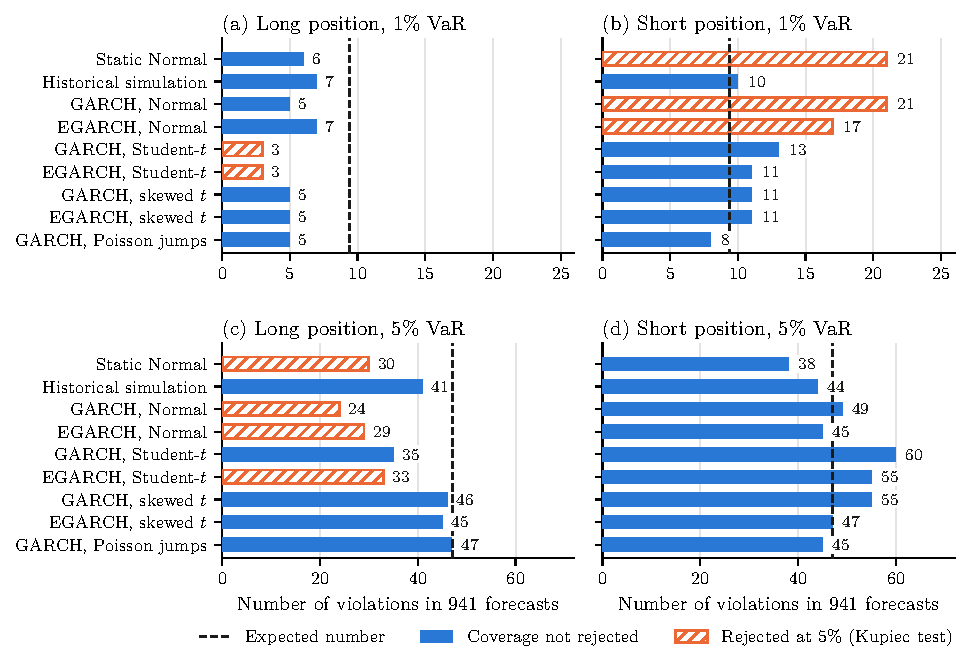
\includegraphics[width=\textwidth]{figures/fig_violations.pdf}
\caption{Number of out-of-sample VaR violations by model. The expected number is \oosExpOne{} at the 1\% level and \oosExpFive{} at the 5\% level. Hatched bars are models whose violation count differs significantly from the expected number (Kupiec test, 5\% level).}\label{fig:viol}
\end{figure}

\begin{figure}[t]
\centering
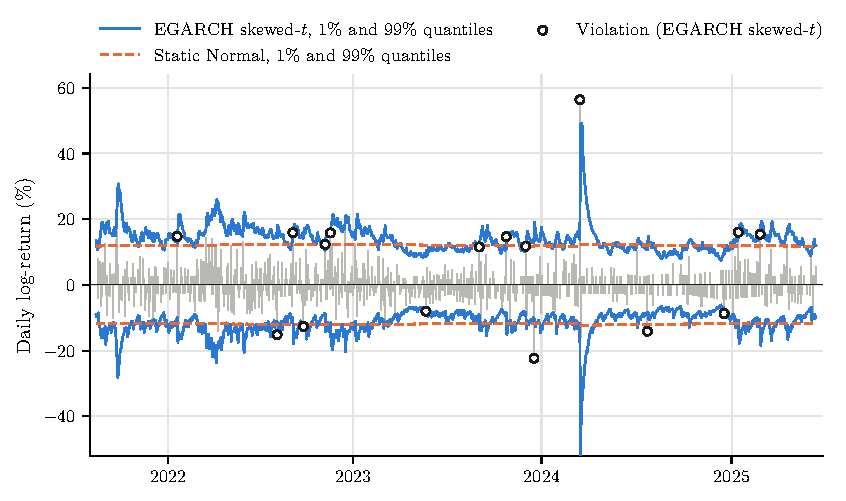
\includegraphics[width=\textwidth]{figures/fig4_oos_var.pdf}
\caption{Out-of-sample 1\% and 99\% quantile forecasts and realised returns, August 2021 to June 2025. Grey bars are daily log-returns. Circles mark the violations of the EGARCH skewed-$t$ model: days on which the return falls outside its band.}\label{fig:oos}
\end{figure}

Table~\ref{tab:oos} reports the backtests, Figure~\ref{fig:viol} summarises the violation counts, and Figure~\ref{fig:oos} plots the forecasts of the preferred model against the static Normal benchmark.

\emph{At the 1\% level, the risk that Gaussian models miss is on the upside.} For a long position, every model produces fewer violations than the \oosExpOne{} expected, and none is rejected for understating risk. For a short position the three Gaussian models produce 17 to 21 violations, about twice the expected number, and are rejected. The Student-$t$, skewed-$t$ and jump models produce 8 to 14.

\emph{Symmetric fat tails over-correct on the downside.} The two symmetric-$t$ models record only four long-side violations at 1\%, significantly fewer than expected ($p_{\mathrm{UC}}=0.040$): they demand more capital against a long position than the data justify. At the 5\% level the Gaussian models are also too conservative on the long side, with 27 to 31 violations against \oosExpFive{} expected, and the symmetric-$t$ models remain so, with 32 and 33. On the short side at the 5\% level the GARCH model with symmetric $t$ errs in the other direction, with 65 violations.

\emph{Models with an asymmetric distribution pass every test.} EGARCH with skewed-$t$ innovations records 6 and 10 violations at 1\% and 49 and 50 at 5\%, with $p$-values above 0.2 throughout. GARCH with skewed $t$ and GARCH with Poisson jumps also pass all eight tests at the 5\% significance level, as does historical simulation, which makes no distributional assumption and therefore reproduces the asymmetry of the data automatically.

\emph{The gain from modelling volatility dynamics is small.} The quantile losses of the better models differ in the third decimal place. A \citet{dieboldmariano1995} test of equal average loss between EGARCH skewed-$t$ and historical simulation gives $t$-statistics between \dmHSROne{} and \dmHSLFive{} across the four tail-and-level combinations, none significant. Against the static Normal, EGARCH skewed-$t$ is significantly better only for the 5\% long-side quantile ($t$-statistic \dmNormalLFive). Figure~\ref{fig:oos} shows why. The conditional band widens after large moves, most visibly after March 2024, but large moves are not preceded by high forecast volatility. On the \violN{} days on which the 1\% or 99\% quantile of the EGARCH skewed-$t$ model was violated, forecast volatility stood on average at the \violSigRank th percentile of its own distribution, and over the whole evaluation period the correlation between the forecast variance and the realised squared return is \corrSigR.

In magnitudes, the average 1\% one-day VaR from the EGARCH skewed-$t$ model over the evaluation period is \avgVarESL\% for a long position and \avgVarESR\% for a short one. The static Normal gives \avgVarNL\% and \avgVarNR\%.

% ------------------------------------------------------------------ 6
\section{Economic interpretation and limitations}\label{sec:disc}

\subsection{Why the fat tail is on the upside}

\emph{The stock as an option on a project.} The equity of any firm can be viewed as a call option on its assets \citep{merton1974}, and a mine that is not yet built adds a second layer: its owner holds the right, but not the obligation, to build it when prices and financing allow \citep{brennanschwartz1985,mcdonaldsiegel1986}. Arafura's value during the sample was almost entirely an option of this kind. The value of an option is convex in the value of what it is written on, and convexity produces a right-skewed distribution: news that the project is more likely to go ahead raises the value of the equity by more than equally sized bad news lowers it. The news that matters most is whether the project will be financed, and it arrives in discrete announcements. On 14 March 2024 a single announcement committed A\$840 million towards a project with a capital cost of about A\$1.7 billion, and the share price rose \jumpSimple\%. Bad news of the same kind is smaller and takes a different form: new shares placed at a discount, as in June 2021 and December 2023 \citep{miningweekly2021,miningweekly2023}, which were followed by two of the three largest one-day falls in the sample. The positive $\hat\gamma$ of Section~\ref{sec:vol} fits the same picture. In most stocks a fall in price raises leverage and with it volatility. For a developer that has so far been financed by share issues that channel is weak, and it is good news about the project that sets off several days of repricing.

\emph{Lottery-type payoffs.} A low-priced stock with high idiosyncratic volatility and positive skewness is what the literature calls a lottery-type stock \citep{kumar2009}. ARU has all three attributes: it traded below A\$0.70 throughout, about \capmIdio\% of the variance of its return is specific to the company, and in \lotShare\% of the months in the sample it recorded at least one daily gain above 10\%. \citet{barberishuang2008} show that investors who overweight small probabilities will pay a premium for such stocks, so that positive skewness is priced and earns a lower average return, and \citet{bali2011} find that stocks with extreme positive daily returns in one month earn low returns in the next. On this view the upside tail documented here is more than a problem of risk measurement. Holders of the stock accept the risk of a long decline in exchange for the chance of a jump, and whoever is short collects a premium for bearing the jump. One stock cannot test whether that premium exists: the mean daily return of \aruMean\% has a standard error of about 0.12\%, so the sample is uninformative about expected returns. But it does identify whose risk a symmetric model misstates.

\emph{What the results mean for a holder of the stock.} The common statement that Gaussian VaR ``underestimates tail risk'' needs a direction attached to it. For ARU the fat tail is the right tail. An investor who is long is, at the 1\% level, adequately or even conservatively covered by a Gaussian model. An investor who is short, or who has sold upside through options, is not: a Gaussian 99\% limit of about 12\% was exceeded twice as often as it should have been, and on one day by a factor of nearly five. The costs described in Section~\ref{sec:arb} compound the problem, since a short position in a stock with a spread of \qSpread\% and little depth cannot be closed quickly on the day of a jump.

\subsection{Limitations}

\emph{What VaR does not measure.} VaR is a quantile and is silent about the size of losses beyond it. On 14 March 2024 the 99\% short-side limit of the preferred model was \esJumpLimit\%, and the realised move was \jumpLog\%. Expected shortfall \citep{artzner1999}, the average loss beyond the VaR, addresses this in principle, but with four to five degrees of freedom its estimate would be driven by a handful of observations. An extreme-value approach to the tail \citep{mcneilfrey2000}, or a jump intensity that rises after a jump \citep{maheumccurdy2004}, would be natural extensions.

\emph{Statistical power.} With \oosN{} forecasts only \oosExpOne{} violations are expected at the 1\% level. Coverage tests have little power against moderate misspecification in samples of this size, so ``not rejected'' is weaker than ``correct''. The 5\% results, with 48 expected violations, are more informative, and they agree with the 1\% results on the role of skewness.

\emph{Data and scope.} The quotes used in Section~\ref{sec:eff} are end-of-day snapshots. Intraday trades and quotes would show the bounce trade by trade and would allow the cost of trading a given size to be measured, and data on securities lending would give the cost of a short position. Neither is used here. Finally, one stock over seven years is a case study. Whether the upside-skewed tail and the weak volatility clustering are general features of pre-production resource companies is an empirical question that this paper does not answer.

% ------------------------------------------------------------------ 7
\section{Conclusion}\label{sec:concl}

This paper examined the daily returns of Arafura Rare Earths from 2018 to 2025 with two questions in mind. On the first, whether returns are predictable, the answer is that they are negatively autocorrelated at one day, robustly in the statistical sense, but that the autocorrelation is the footprint of a price grid in which one tick is about 2\% of the price. The closing price sits at the bid or the ask on most days, the autocorrelation is insignificant in returns measured at quote mid-points, and a rule that trades on it loses money at the quoted spread. The evidence does not contradict weak-form efficiency.

On the second, how to measure the stock's one-day risk, the innovation distribution matters more than the volatility recursion. Innovations have four to five degrees of freedom and a longer right tail than left, the profile of an equity that is an option on a project not yet financed. Models that ignore the fat tails understate the risk of a short position, models that add fat tails symmetrically overstate the risk of a long one, and models with an asymmetric distribution, whether a skewed Student-$t$ or a Poisson mixture with positive mean jump, are correctly calibrated in both directions. A simple historical-simulation quantile does as well out of sample, which says that for this stock the unconditional shape of the distribution carries most of the information and conditional volatility relatively little.

For risk management in junior resource stocks more generally, the results suggest three checks before a VaR model is trusted: whether apparent return predictability survives the bid--ask spread, whether the two tails have been examined separately, and whether the model has been tested on data it has not seen.

% ------------------------------------------------------------------ refs
\clearpage
\phantomsection\addcontentsline{toc}{section}{References}
\bibliographystyle{apalike}
\bibliography{refs}


% ------------------------------------------------------------------ disclosure
\section*{Statement of contributions}
{\small The empirical work on which this paper is based was carried out during the internship by Dr.\ Roman Mestre and me together. He taught me the concepts and methods, and we jointly collected and cleaned the data and estimated the market-model tests and the GARCH and EGARCH models with Normal and Student-$t$ innovations. I wrote the paper, both the first version (December 2025) and this revision. Dr.\ Mestre did not take part in writing either version.\par}

\section*{Declaration of generative AI use}
{\small The first version of this paper (December 2025) and the empirical work described above, including the market-model tests and the GARCH and EGARCH models with Normal and Student-$t$ innovations, predate this revision. In this revision I used Claude (Anthropic) to extend the analysis, including the skewed Student-$t$ and Poisson jump models; to produce figures and tables; and to help draft text. I take full responsibility for the content of this paper, and all errors are my own.\par}

% ------------------------------------------------------------------ appendix
\clearpage
\phantomsection\addcontentsline{toc}{section}{Appendix}
\addtocontents{toc}{\protect\setcounter{tocdepth}{0}}
\appendix
\numberwithin{equation}{section}

\section{Expected absolute value of the innovation}\label{app:absz}

The EGARCH equation~\eqref{eq:egarch} is centred with $\E|z_t|$, which depends on the distribution.

\emph{Normal.} Since the density is symmetric,
\begin{equation}
\E|z|=2\int_{0}^{\infty}\frac{z}{\sqrt{2\pi}}\,e^{-z^{2}/2}\,dz=\frac{2}{\sqrt{2\pi}}\Bigl[-e^{-z^{2}/2}\Bigr]_{0}^{\infty}=\sqrt{\frac{2}{\pi}}\approx 0.798 .
\end{equation}

\emph{Student-$t$.} Let $c_\nu=\Gamma\!\left(\frac{\nu+1}{2}\right)\big/\bigl[\sqrt{\pi(\nu-2)}\,\Gamma\!\left(\frac{\nu}{2}\right)\bigr]$ be the constant in~\eqref{eq:t}. With the substitution $u=1+z^{2}/(\nu-2)$, so that $z\,dz=\frac{\nu-2}{2}\,du$,
\begin{equation}
\E|z|=2c_\nu\int_{0}^{\infty}z\left(1+\frac{z^{2}}{\nu-2}\right)^{-\frac{\nu+1}{2}}dz
=c_\nu(\nu-2)\int_{1}^{\infty}u^{-\frac{\nu+1}{2}}\,du=\frac{2c_\nu(\nu-2)}{\nu-1},
\end{equation}
that is,
\begin{equation}
\E|z|=\frac{2\sqrt{\nu-2}\;\Gamma\!\left(\frac{\nu+1}{2}\right)}{\sqrt{\pi}\,(\nu-1)\,\Gamma\!\left(\frac{\nu}{2}\right)} ,
\end{equation}
which tends to $\sqrt{2/\pi}$ as $\nu\to\infty$ and equals 0.72 at $\nu=4.5$. Replacing $\E|z|$ by a different constant $m$ in~\eqref{eq:egarch} changes $\omega$ to $\omega+\alpha(m-\E|z|)$ and leaves every other parameter, the fitted variances and the likelihood unchanged.

\section{Test statistics}\label{app:tests}

\emph{Robust autocorrelations.} Let $x_t=r_t-\bar r$. If $x_t$ is unpredictable from its past but has time-varying variance, $\sqrt{T}\hat\rho_k$ is asymptotically Normal with variance $\delta_k$, estimated by \citep{lomackinlay1988}
\begin{equation}
\hat\delta_k=\frac{T\sum_{t=k+1}^{T}x_t^2x_{t-k}^2}{\bigl(\sum_{t=1}^{T}x_t^2\bigr)^{2}},\qquad t^{*}_k=\frac{\hat\rho_k}{\sqrt{\hat\delta_k/T}} .
\end{equation}
Under independence $\delta_k=1$ and $t_k^{*}$ reduces to $\sqrt{T}\hat\rho_k$. The robust portmanteau statistic is $Q^{*}(m)=\sum_{k=1}^{m}(t_k^{*})^2$, asymptotically $\chi^2(m)$ \citep{lobato2001}.

\emph{Variance ratio.} With $\hat\sigma^2(q)$ the variance of overlapping $q$-day returns divided by $q$, corrected for bias as in \citet{lomackinlay1988}, $\VR(q)=\hat\sigma^2(q)/\hat\sigma^2(1)$ and
\begin{equation}
z(q)=\frac{\VR(q)-1}{\sqrt{2(2q-1)(q-1)/(3qT)}},\qquad
z^{*}(q)=\frac{\VR(q)-1}{\sqrt{\hat\theta(q)/T}},\qquad
\hat\theta(q)=\sum_{j=1}^{q-1}\left[\frac{2(q-j)}{q}\right]^{2}\hat\delta_j .
\end{equation}

\emph{Independence of violations.} Let $I_t$ equal one on a violation day and $n_{ij}$ be the number of days on which $I_{t-1}=i$ and $I_t=j$, with $\hat\pi=(n_{01}+n_{11})/T$, $\hat\pi_{01}=n_{01}/(n_{00}+n_{01})$ and $\hat\pi_{11}=n_{11}/(n_{10}+n_{11})$. The statistic of \citet{christoffersen1998} compares the frequency of violations after a violation, $\hat\pi_{11}$, with the frequency after a normal day, $\hat\pi_{01}$:
\begin{equation}
LR_{\mathrm{IND}}=-2\ln\frac{(1-\hat\pi)^{n_{00}+n_{10}}\hat\pi^{\,n_{01}+n_{11}}}{(1-\hat\pi_{01})^{n_{00}}\hat\pi_{01}^{\,n_{01}}(1-\hat\pi_{11})^{n_{10}}\hat\pi_{11}^{\,n_{11}}}\;\sim\;\chi^2(1).
\end{equation}
The conditional-coverage statistic is $LR_{\mathrm{CC}}=LR_{\mathrm{UC}}+LR_{\mathrm{IND}}\sim\chi^2(2)$.

\emph{Jump probabilities and quantiles.} In the jump model of Section~\ref{sec:jump}, write $w_n=e^{-\kappa}\kappa^{n}/n!$ and let $\varphi_n(\varepsilon_t)$ be the Normal density with mean $(n-\kappa)\theta$ and variance $h_t+n\delta^2$. The probability that at least one jump occurred on day $t$ is, by Bayes' rule,
\begin{equation}
\Pr(N_t\ge 1\mid r_t)=1-\frac{w_0\,\varphi_0(\varepsilon_t)}{\sum_{n\ge0}w_n\,\varphi_n(\varepsilon_t)} ,
\end{equation}
and the $p$-quantile $x$ of $\varepsilon_t$ solves $\sum_{n\ge0}w_n\,\Phi\bigl((x-(n-\kappa)\theta)/\sqrt{h_t+n\delta^2}\bigr)=p$.

\end{document}
